% ============================================================================
% DARIJA-VOICE MED - Scientific Poster A0
% Spring School - AI For Impact | École Centrale Casablanca
% ============================================================================

\documentclass[a0paper,portrait]{a0poster}

% ----- Packages -----
\usepackage[utf8]{inputenc}
\usepackage[T1]{fontenc}
\usepackage{graphicx}
\usepackage{xcolor}
\usepackage{tikz}
\usepackage{tcolorbox}
\usepackage{multicol}
\usepackage{enumitem}
\usepackage{booktabs}
\usepackage{array}
\usepackage{tabularx}
\usepackage{fontawesome5}
\usepackage{qrcode}
\usepackage{geometry}
\usepackage{helvet}
\renewcommand{\familydefault}{\sfdefault}

% ----- Page Geometry -----
\geometry{
    paperwidth=841mm,
    paperheight=1189mm,
    left=20mm,
    right=20mm,
    top=20mm,
    bottom=20mm
}

% ----- Color Scheme (Purple, Sky Blue, White) -----
\definecolor{primarypurple}{RGB}{102, 51, 153}
\definecolor{secondarypurple}{RGB}{138, 92, 179}
\definecolor{skyblue}{RGB}{135, 206, 235}
\definecolor{lightskyblue}{RGB}{200, 230, 250}
\definecolor{darktext}{RGB}{33, 33, 33}
\definecolor{accentgreen}{RGB}{46, 204, 113}
\definecolor{accentorange}{RGB}{243, 156, 18}
\definecolor{accentred}{RGB}{231, 76, 60}

% ----- TColorBox Styles -----
\tcbset{
    boxstyle/.style={
        colback=white,
        colframe=primarypurple,
        boxrule=3pt,
        arc=10pt,
        left=15pt,
        right=15pt,
        top=15pt,
        bottom=15pt,
        fonttitle=\bfseries\Huge\color{white},
        coltitle=white,
        colbacktitle=primarypurple,
        toptitle=10pt,
        bottomtitle=10pt,
    },
    contributionbox/.style={
        colback=lightskyblue,
        colframe=skyblue,
        boxrule=3pt,
        arc=10pt,
        left=15pt,
        right=15pt,
        top=15pt,
        bottom=15pt,
        fonttitle=\bfseries\Huge\color{darktext},
        coltitle=darktext,
        colbacktitle=skyblue,
        toptitle=10pt,
        bottomtitle=10pt,
    }
}

\begin{document}

% ----- Background -----
\begin{tikzpicture}[remember picture, overlay]
    \fill[white] (current page.south west) rectangle (current page.north east);
    % Decorative header gradient
    \shade[top color=primarypurple, bottom color=secondarypurple] 
        ([yshift=-180mm]current page.north west) rectangle (current page.north east);
    % Decorative footer
    \fill[primarypurple] (current page.south west) rectangle ([yshift=60mm]current page.south east);
\end{tikzpicture}

% ============================================================================
% HEADER
% ============================================================================
\begin{tikzpicture}[remember picture, overlay]
    % Title
    \node[anchor=north, text=white, font=\fontsize{100}{120}\selectfont\bfseries] 
        at ([yshift=-40mm]current page.north) {DARIJA-VOICE MED};
    
    % Subtitle
    \node[anchor=north, text=white, font=\fontsize{50}{60}\selectfont] 
        at ([yshift=-100mm]current page.north) {Privacy-Preserving AI Health Assistant for Rural Morocco};
    
    % Authors
    \node[anchor=north, text=white, font=\fontsize{36}{44}\selectfont] 
        at ([yshift=-145mm]current page.north) {
            \textbf{KAMBIRE Eric} \quad \& \quad \textbf{MAIGA Jamil Claude}
        };
    
    % Affiliation
    \node[anchor=north, text=lightskyblue, font=\fontsize{30}{36}\selectfont\itshape] 
        at ([yshift=-175mm]current page.north) {École Centrale Casablanca};
    
    % Logo placeholder (left)
    \node[anchor=north west] at ([xshift=30mm, yshift=-30mm]current page.north west) {
        \begin{tcolorbox}[colback=white, colframe=white, boxrule=0pt, width=150mm, height=80mm, valign=center, halign=center]
            \fontsize{24}{28}\selectfont\bfseries\color{primarypurple}
            Spring School\\AI For Impact
        \end{tcolorbox}
    };
    
    % Morocco Flag Icon (right)
    \node[anchor=north east, text=white, font=\fontsize{80}{90}\selectfont] 
        at ([xshift=-40mm, yshift=-60mm]current page.north east) {\faHospital};
\end{tikzpicture}

\vspace{200mm}

% ============================================================================
% MAIN CONTENT - Two Columns
% ============================================================================
\begin{multicols}{2}

% ----- LEFT COLUMN -----

% === INTRODUCTION & OBJECTIVES ===
\begin{tcolorbox}[boxstyle, title={\faExclamationTriangle \quad Introduction \& Objectives}]

\textbf{\LARGE\color{primarypurple} Problem Statement}
\vspace{5mm}

\begin{itemize}[leftmargin=*, itemsep=8pt, font=\Large]
    \item[\faUsers] \textbf{30\% of rural Moroccan population} is illiterate
    \item[\faUserMd] \textbf{1 doctor per 3,000 inhabitants} in rural areas
    \item[\faLanguage] \textbf{Language barrier:} Patients only speak Darija
    \item[\faWifi] \textbf{Low connectivity:} No stable internet in remote regions
\end{itemize}

\vspace{10mm}
\textbf{\LARGE\color{primarypurple} Research Objectives}
\vspace{5mm}

\begin{itemize}[leftmargin=*, itemsep=8pt, font=\Large]
    \item[\faCheckCircle] Build a maternal health assistant with \textbf{Darija voice input}
    \item[\faCheckCircle] Ensure \textbf{data privacy} through Federated Learning
    \item[\faCheckCircle] Provide \textbf{audio responses} for illiterate patients
    \item[\faCheckCircle] Enable \textbf{pre-diagnosis} accessible without a doctor
\end{itemize}

\end{tcolorbox}

\vspace{20mm}

% === MAIN CONTRIBUTION ===
\begin{tcolorbox}[contributionbox, title={\faStar \quad Main Contribution}]

\begin{center}
\textbf{\Huge\color{primarypurple} Social Impact: Healthcare Accessible to All}
\end{center}

\vspace{10mm}

\renewcommand{\arraystretch}{1.8}
\begin{tabularx}{\linewidth}{>{\bfseries\large}l X}
\toprule
\textbf{Innovation} & \textbf{Impact} \\
\midrule
\faVolumeUp\ Darija Voice Interface & Eliminates literacy barrier \\
\faHeadphones\ TTS Audio Response & Patient HEARS medical advice \\
\faShieldAlt\ Federated Learning & Data NEVER leaves the device \\
\faLock\ Differential Privacy & Mathematical protection $\varepsilon=1.0$ \\
\bottomrule
\end{tabularx}

\vspace{15mm}

\begin{center}
\begin{tcolorbox}[colback=white, colframe=accentgreen, boxrule=2pt, width=0.95\linewidth]
\Large\centering
\textbf{\color{accentgreen}\faLightbulb\ First-of-its-kind:}\\[5mm]
\large
$\bullet$ First Darija voice health system with audio response\\
$\bullet$ Federated Learning on Moroccan maternal data\\
$\bullet$ \textbf{250$\times$ less data transmitted} vs traditional cloud
\end{tcolorbox}
\end{center}

\end{tcolorbox}

\vspace{20mm}

% === TECHNICAL PIPELINE ===
\begin{tcolorbox}[boxstyle, title={\faCogs \quad Technical Pipeline}]

\begin{center}
\begin{tikzpicture}[scale=1.2, transform shape,
    block/.style={rectangle, draw=primarypurple, fill=lightskyblue, 
                  text width=8em, text centered, rounded corners, 
                  minimum height=4em, font=\large\bfseries},
    arrow/.style={->, >=stealth, line width=2pt, color=primarypurple}]
    
    \node[block] (audio) at (0,0) {\faMicrophone\\Audio Input};
    \node[block] (asr) at (5,0) {\faFileAlt\\ASR Whisper\\Darija};
    \node[block] (slm) at (10,0) {\faBrain\\MedGemma\\4B};
    \node[block] (fl) at (5,-4) {\faProjectDiagram\\XGBoost FL\\Prediction};
    \node[block] (tts) at (10,-4) {\faVolumeUp\\TTS Darija\\Audio};
    
    \draw[arrow] (audio) -- (asr);
    \draw[arrow] (asr) -- (slm);
    \draw[arrow] (slm) -- (fl);
    \draw[arrow] (fl) -- (tts);
\end{tikzpicture}
\end{center}

\vspace{10mm}

\renewcommand{\arraystretch}{1.6}
\begin{tabularx}{\linewidth}{>{\bfseries}l l X}
\toprule
\textbf{Component} & \textbf{Technology} & \textbf{Role} \\
\midrule
ASR & whisper-small-darija & Moroccan voice transcription \\
SLM & MedGemma-4B (Google) & Specialized medical analysis \\
FL & Flower + XGBoost & Distributed federated learning \\
TTS & gTTS (Arabic) & Darija speech synthesis \\
Privacy & Differential Privacy & Noise injection $\varepsilon=1.0$ \\
\bottomrule
\end{tabularx}

\end{tcolorbox}

\columnbreak

% ----- RIGHT COLUMN -----

% === METHODOLOGY & ARCHITECTURE ===
\begin{tcolorbox}[boxstyle, title={\faNetworkWired \quad Methodology \& Architecture}]

\textbf{\LARGE\color{primarypurple} Federated Learning Architecture}
\vspace{10mm}

\begin{center}
\begin{tikzpicture}[scale=1.0, transform shape,
    village/.style={rectangle, draw=secondarypurple, fill=lightskyblue,
                    text width=10em, text centered, rounded corners,
                    minimum height=6em, font=\large},
    server/.style={rectangle, draw=primarypurple, fill=primarypurple,
                   text width=12em, text centered, rounded corners,
                   minimum height=5em, font=\large\bfseries, text=white},
    arrow/.style={->, >=stealth, line width=2pt, color=secondarypurple}]
    
    \node[village] (v1) at (0,0) {\faHome\ \textbf{Village 1}\\(Non-IID)\\Client 1};
    \node[village] (v2) at (6,0) {\faHome\ \textbf{Village 2}\\(Non-IID)\\Client 2};
    \node[village] (v3) at (12,0) {\faHome\ \textbf{Village 3}\\(Non-IID)\\Client 3};
    \node[server] (srv) at (6,-6) {\faServer\ Flower Server\\FedAvg Aggregation};
    
    \draw[arrow] (v1.south) -- node[left, font=\small, text=darktext] {noisy params} (srv.north west);
    \draw[arrow] (v2.south) -- (srv.north);
    \draw[arrow] (v3.south) -- node[right, font=\small, text=darktext] {noisy params} (srv.north east);
    
    \node[font=\Large\color{accentgreen}] at (6,-3) {\faLock\ NO RAW DATA TRANSMITTED};
\end{tikzpicture}
\end{center}

\vspace{10mm}

\textbf{\LARGE\color{primarypurple} Privacy Guarantees}
\vspace{5mm}

\begin{itemize}[leftmargin=*, itemsep=6pt, font=\Large]
    \item[\faCheckCircle] \textbf{Audio:} Processed locally, never sent to server
    \item[\faCheckCircle] \textbf{Symptoms:} Extracted and stored locally only
    \item[\faCheckCircle] \textbf{Medical Images:} Analyzed locally, never uploaded
    \item[\faCheckCircle] \textbf{Model params:} Noised with Differential Privacy ($\varepsilon=1.0$)
\end{itemize}

\end{tcolorbox}

\vspace{20mm}

% === RESULTS ===
\begin{tcolorbox}[boxstyle, title={\faChartBar \quad Results \& Performance}]

\textbf{\LARGE\color{primarypurple} Performance Metrics}
\vspace{10mm}

\begin{center}
\renewcommand{\arraystretch}{2.0}
\begin{tabular}{>{\bfseries\Large}l >{\Large}c >{\Large}l}
\toprule
\textbf{Metric} & \textbf{Value} & \textbf{Benchmark} \\
\midrule
FL Accuracy & \textcolor{accentgreen}{\textbf{85\%+}} & vs 82\% centralized \\
Data Reduction & \textcolor{accentgreen}{\textbf{250$\times$}} & vs cloud \\
Privacy Budget $\varepsilon$ & \textcolor{accentgreen}{\textbf{1.0}} & Gold standard \\
TTS Latency & \textcolor{accentgreen}{\textbf{<2s}} & Real-time \\
VRAM Usage & \textcolor{accentgreen}{\textbf{$\sim$3 GB}} & T4 compatible \\
\bottomrule
\end{tabular}
\end{center}

\vspace{15mm}

\textbf{\LARGE\color{primarypurple} Dataset Information}
\vspace{5mm}

\begin{itemize}[leftmargin=*, itemsep=6pt, font=\Large]
    \item[\faDatabase] \textbf{Source:} UCI Maternal Health Risk (1,014 samples)
    \item[\faMapMarkerAlt] \textbf{Distribution:} Non-IID across 3 simulated villages
    \item[\faTags] \textbf{Classes:} High Risk, Mid Risk, Low Risk
    \item[\faList] \textbf{Features:} SystolicBP, DiastolicBP, BloodSugar, BodyTemp, HeartRate, Age
\end{itemize}

\end{tcolorbox}

\vspace{20mm}

% === CONCLUSION ===
\begin{tcolorbox}[contributionbox, title={\faFlagCheckered \quad Conclusion \& Future Work}]

\textbf{\LARGE\color{primarypurple} Impact Summary}
\vspace{5mm}

\renewcommand{\arraystretch}{1.6}
\begin{tabularx}{\linewidth}{X c l}
\toprule
\textbf{Objective} & \textbf{Status} & \textbf{Beneficiary} \\
\midrule
Darija voice diagnosis & \textcolor{accentgreen}{\faCheckCircle} & Rural patient \\
Audio response & \textcolor{accentgreen}{\faCheckCircle} & Illiterate patient \\
Prescription translation & \textcolor{accentgreen}{\faCheckCircle} & Patient/Health worker \\
Privacy guaranteed & \textcolor{accentgreen}{\faCheckCircle} & Everyone \\
\bottomrule
\end{tabularx}

\vspace{10mm}

\textbf{\LARGE\color{primarypurple} Future Developments}
\vspace{5mm}

\begin{multicols}{2}
\begin{itemize}[leftmargin=*, itemsep=4pt, font=\large]
    \item[\faTabletAlt] Offline Android deployment
    \item[\faGlobe] Amazigh dialect extension
    \item[\faHospitalAlt] RAMED integration
    \item[\faStethoscope] Clinical validation with CHUs
\end{itemize}
\end{multicols}

\vspace{5mm}

\begin{center}
\begin{tcolorbox}[colback=primarypurple!10, colframe=primarypurple, boxrule=2pt, width=0.95\linewidth]
\Large\centering\itshape
\textcolor{primarypurple}{"Reduce maternal mortality by 15\% in rural Morocco by 2030\\through accessible pre-diagnosis."}
\end{tcolorbox}
\end{center}

\end{tcolorbox}

\end{multicols}

% ============================================================================
% FOOTER
% ============================================================================
\begin{tikzpicture}[remember picture, overlay]
    % References (left)
    \node[anchor=south west, text=white, font=\large, align=left] 
        at ([xshift=30mm, yshift=15mm]current page.south west) {
            \textbf{\Large References:}\\[3mm]
            [1] McMahan et al. (2017). Communication-Efficient Learning from Decentralized Data\\
            [2] Dwork \& Roth (2014). The Algorithmic Foundations of Differential Privacy\\
            [3] Google Health (2024). MedGemma: Medical Foundation Models
        };
    
    % GitHub Link (center)
    \node[anchor=south, text=white, font=\Large] 
        at ([yshift=25mm]current page.south) {
            \faGithub\ \textbf{github.com/Eric-Kambire/AgorAI}
        };
    
    % QR Code placeholder (right)
    \node[anchor=south east] at ([xshift=-40mm, yshift=10mm]current page.south east) {
        \begin{tcolorbox}[colback=white, colframe=white, boxrule=0pt, width=50mm]
            \centering
            \qrcode[height=40mm]{https://github.com/Eric-Kambire/AgorAI}
        \end{tcolorbox}
    };
    
    % Event name
    \node[anchor=south, text=lightskyblue, font=\large\itshape] 
        at ([yshift=5mm]current page.south) {
            Spring School - AI For Impact | École Centrale Casablanca | 2026
        };
\end{tikzpicture}

\end{document}
